\documentclass{article}
\usepackage{tikz}


\definecolor{myorange}{RGB}{229, 152, 102 }
\definecolor{myviolet}{RGB}{165, 105, 189}
\definecolor{myblue}{RGB}{21, 67, 96}
\definecolor{myback}{RGB}{214,234,248}



\newtheorem{theorem}{Theorem}[section]

\title{Pythagorean Theorem}
\author{1505069}
\date{\today}

\begin{document}
\maketitle
\section{Introduction}
In this document, we present the very famous theorem in mathematics
\textit{Pythagorean theorem}, which is stated as follows.
\begin{theorem}[Pythagorean theorem]
The square of the hypotenuse (the side opposite the right angle) is equal to the sum of the squares of the other two sides.
\end{theorem}

Numerous mathematicians proposed various proofs to the theorem. The
theorem was long known even before the time of Pythagoras. Pythagoras was
the first to provide with a sound proof. The proof that Pythagoras gave was by rearrangement. Even the great Albert Einstein also proved the theorem without rearrangement, rather by using dissection. Figure \ref{fig:representation1} shows the visual representation of the theorem.
\begin{figure}[h]
    \centering
    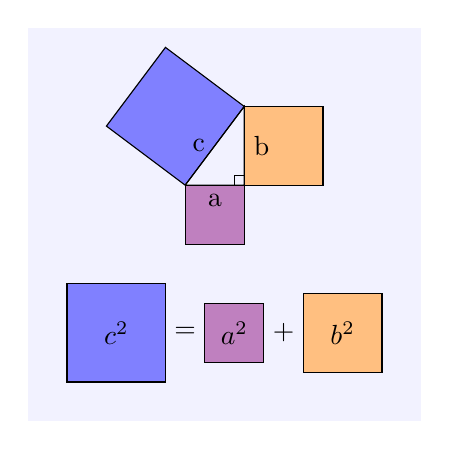
\begin{tikzpicture}[scale=.25]
   %\draw[help lines] (0,0) grid (20,20);
    \path[fill=blue!5]  (0,0) rectangle (20,20);
   	\draw[fill=orange!50] (11,12) rectangle (15,16) ;
     \draw[fill=violet!50] (8,12) rectangle (11,9);
   	\begin{scope}[xshift=8cm,yshift=12cm]
		\draw[rotate={asin(4/5)}] [fill=blue!50] (0,0) rectangle (5,5);
	\end{scope}
    \draw (8,12)--  node[below] {a}(11,12)-- node[right] {b}(11,16)-- node[left] {c}(8,12);
    \draw (10.5,12) --(10.5,12.5)--(11,12.5);
    \draw[fill=blue!50] (2,2) rectangle (7,7) ;
	 \draw[fill=violet!50] (9,3) rectangle (12,6);
	 \draw[fill=orange!50] (14,2.5) rectangle (18,6.5) ;
	  \node at (4.5,4.5) {$c^2$};
	 \node at (8,4.5) {$=$};
	 \node at (10.5,4.5) {$a^2$};
	  \node at (13,4.5) {$+$};
	   \node at (16,4.5) {$b^2$};

    
  	\end{tikzpicture}
	\caption{Visual representation of the famous Pythagorean theorem.}
    \label{fig:representation1}
\end{figure}


\begin{figure}[h]
    \centering
    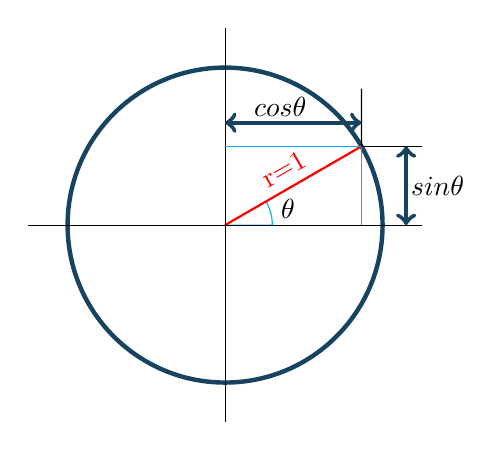
\begin{tikzpicture}[scale=2][>=stealth]
  		\draw[ultra thick,myblue] (0,0) circle (1cm);
		\draw[cyan] (0,0) -- (3mm,0mm) arc (0:30:3mm) -- cycle ;
		\node at (4mm,1mm) {$\theta$};
		\draw[thick,red] (0,0) -- node[above,sloped] {r=1} (30:1cm) ;
		 \draw[-] (-1.25,0) -- (1.25,0) coordinate (x axis);
 		\draw[-] (0,-1.25) -- (0,1.25) coordinate (y axis);
		\draw[cyan] (30:1cm) -- (30:1cm |- x axis);
		\draw[cyan] (30:1cm -| y axis) -- (30:1cm);
		\draw[black] (30:1cm ) -- (30:1cm -| x axis) ;
		\draw  (30:1cm )  -- ({sqrt(.75)},{sqrt(.75)});
		\draw[<->,ultra thick,myblue] (1.15,0)--  (1.15,.5);
		\draw[<->,ultra thick,myblue] (0,.65)--  ({sqrt(.75)},.65);
		\node  at (.35,.75) {$cos \theta$};
		\node  at (1.35,.25) {$sin \theta$};
	\end{tikzpicture}
	\caption{Alternate representation of Pythagorean theorem.}
	\label{fig:representation2}
\end{figure}

\section{Trigonometric Forms}
Lots of other forms of the same theorem exist. The most useful, perhaps, are
expressed in trigonometric terms, as follows:
\begin{equation}
sin^2\theta  + cos^2\theta  =1
\label{equ:equation1}
\end{equation}
\begin{equation}
sec^2\theta  - tan^2\theta  =1
\label{equ:equation2}
\end{equation}
\begin{equation}
cosec^2\theta  - cot^2\theta  =1
\label{equ:equation3}
\end{equation}
\subsection{Representing the First}
Taking \ref{equ:equation1}, we can show them as shown in Figure\ref{fig:representation2}. When we take a point at unit distance from the origin, the y and x co-ordinates become $sin \theta$ and $cos \theta$ respectively. Therefore, sum of the squares of the two becomes equal to the square of the unit distance, which of course, is 1.
\end{document}
